% Options for packages loaded elsewhere
\PassOptionsToPackage{unicode}{hyperref}
\PassOptionsToPackage{hyphens}{url}
%
\documentclass[
]{article}
\usepackage{amsmath,amssymb}
\usepackage{lmodern}
\usepackage{iftex}
\ifPDFTeX
  \usepackage[T1]{fontenc}
  \usepackage[utf8]{inputenc}
  \usepackage{textcomp} % provide euro and other symbols
\else % if luatex or xetex
  \usepackage{unicode-math}
  \defaultfontfeatures{Scale=MatchLowercase}
  \defaultfontfeatures[\rmfamily]{Ligatures=TeX,Scale=1}
\fi
% Use upquote if available, for straight quotes in verbatim environments
\IfFileExists{upquote.sty}{\usepackage{upquote}}{}
\IfFileExists{microtype.sty}{% use microtype if available
  \usepackage[]{microtype}
  \UseMicrotypeSet[protrusion]{basicmath} % disable protrusion for tt fonts
}{}
\makeatletter
\@ifundefined{KOMAClassName}{% if non-KOMA class
  \IfFileExists{parskip.sty}{%
    \usepackage{parskip}
  }{% else
    \setlength{\parindent}{0pt}
    \setlength{\parskip}{6pt plus 2pt minus 1pt}}
}{% if KOMA class
  \KOMAoptions{parskip=half}}
\makeatother
\usepackage{xcolor}
\IfFileExists{xurl.sty}{\usepackage{xurl}}{} % add URL line breaks if available
\IfFileExists{bookmark.sty}{\usepackage{bookmark}}{\usepackage{hyperref}}
\hypersetup{
  pdftitle={Untitled},
  hidelinks,
  pdfcreator={LaTeX via pandoc}}
\urlstyle{same} % disable monospaced font for URLs
\usepackage[margin=1in]{geometry}
\usepackage{color}
\usepackage{fancyvrb}
\newcommand{\VerbBar}{|}
\newcommand{\VERB}{\Verb[commandchars=\\\{\}]}
\DefineVerbatimEnvironment{Highlighting}{Verbatim}{commandchars=\\\{\}}
% Add ',fontsize=\small' for more characters per line
\usepackage{framed}
\definecolor{shadecolor}{RGB}{248,248,248}
\newenvironment{Shaded}{\begin{snugshade}}{\end{snugshade}}
\newcommand{\AlertTok}[1]{\textcolor[rgb]{0.94,0.16,0.16}{#1}}
\newcommand{\AnnotationTok}[1]{\textcolor[rgb]{0.56,0.35,0.01}{\textbf{\textit{#1}}}}
\newcommand{\AttributeTok}[1]{\textcolor[rgb]{0.77,0.63,0.00}{#1}}
\newcommand{\BaseNTok}[1]{\textcolor[rgb]{0.00,0.00,0.81}{#1}}
\newcommand{\BuiltInTok}[1]{#1}
\newcommand{\CharTok}[1]{\textcolor[rgb]{0.31,0.60,0.02}{#1}}
\newcommand{\CommentTok}[1]{\textcolor[rgb]{0.56,0.35,0.01}{\textit{#1}}}
\newcommand{\CommentVarTok}[1]{\textcolor[rgb]{0.56,0.35,0.01}{\textbf{\textit{#1}}}}
\newcommand{\ConstantTok}[1]{\textcolor[rgb]{0.00,0.00,0.00}{#1}}
\newcommand{\ControlFlowTok}[1]{\textcolor[rgb]{0.13,0.29,0.53}{\textbf{#1}}}
\newcommand{\DataTypeTok}[1]{\textcolor[rgb]{0.13,0.29,0.53}{#1}}
\newcommand{\DecValTok}[1]{\textcolor[rgb]{0.00,0.00,0.81}{#1}}
\newcommand{\DocumentationTok}[1]{\textcolor[rgb]{0.56,0.35,0.01}{\textbf{\textit{#1}}}}
\newcommand{\ErrorTok}[1]{\textcolor[rgb]{0.64,0.00,0.00}{\textbf{#1}}}
\newcommand{\ExtensionTok}[1]{#1}
\newcommand{\FloatTok}[1]{\textcolor[rgb]{0.00,0.00,0.81}{#1}}
\newcommand{\FunctionTok}[1]{\textcolor[rgb]{0.00,0.00,0.00}{#1}}
\newcommand{\ImportTok}[1]{#1}
\newcommand{\InformationTok}[1]{\textcolor[rgb]{0.56,0.35,0.01}{\textbf{\textit{#1}}}}
\newcommand{\KeywordTok}[1]{\textcolor[rgb]{0.13,0.29,0.53}{\textbf{#1}}}
\newcommand{\NormalTok}[1]{#1}
\newcommand{\OperatorTok}[1]{\textcolor[rgb]{0.81,0.36,0.00}{\textbf{#1}}}
\newcommand{\OtherTok}[1]{\textcolor[rgb]{0.56,0.35,0.01}{#1}}
\newcommand{\PreprocessorTok}[1]{\textcolor[rgb]{0.56,0.35,0.01}{\textit{#1}}}
\newcommand{\RegionMarkerTok}[1]{#1}
\newcommand{\SpecialCharTok}[1]{\textcolor[rgb]{0.00,0.00,0.00}{#1}}
\newcommand{\SpecialStringTok}[1]{\textcolor[rgb]{0.31,0.60,0.02}{#1}}
\newcommand{\StringTok}[1]{\textcolor[rgb]{0.31,0.60,0.02}{#1}}
\newcommand{\VariableTok}[1]{\textcolor[rgb]{0.00,0.00,0.00}{#1}}
\newcommand{\VerbatimStringTok}[1]{\textcolor[rgb]{0.31,0.60,0.02}{#1}}
\newcommand{\WarningTok}[1]{\textcolor[rgb]{0.56,0.35,0.01}{\textbf{\textit{#1}}}}
\usepackage{longtable,booktabs,array}
\usepackage{calc} % for calculating minipage widths
% Correct order of tables after \paragraph or \subparagraph
\usepackage{etoolbox}
\makeatletter
\patchcmd\longtable{\par}{\if@noskipsec\mbox{}\fi\par}{}{}
\makeatother
% Allow footnotes in longtable head/foot
\IfFileExists{footnotehyper.sty}{\usepackage{footnotehyper}}{\usepackage{footnote}}
\makesavenoteenv{longtable}
\usepackage{graphicx}
\makeatletter
\def\maxwidth{\ifdim\Gin@nat@width>\linewidth\linewidth\else\Gin@nat@width\fi}
\def\maxheight{\ifdim\Gin@nat@height>\textheight\textheight\else\Gin@nat@height\fi}
\makeatother
% Scale images if necessary, so that they will not overflow the page
% margins by default, and it is still possible to overwrite the defaults
% using explicit options in \includegraphics[width, height, ...]{}
\setkeys{Gin}{width=\maxwidth,height=\maxheight,keepaspectratio}
% Set default figure placement to htbp
\makeatletter
\def\fps@figure{htbp}
\makeatother
\setlength{\emergencystretch}{3em} % prevent overfull lines
\providecommand{\tightlist}{%
  \setlength{\itemsep}{0pt}\setlength{\parskip}{0pt}}
\setcounter{secnumdepth}{5}
\usepackage{subfig}
\ifLuaTeX
  \usepackage{selnolig}  % disable illegal ligatures
\fi

\title{Untitled}
\author{}
\date{\vspace{-2.5em}2022-06-11}

\begin{document}
\maketitle

{
\setcounter{tocdepth}{2}
\tableofcontents
}
\hypertarget{r-markdown}{%
\subsection{R Markdown}\label{r-markdown}}

\begin{Shaded}
\begin{Highlighting}[]
\NormalTok{EViews\textgreater{} wfcreate(wf=sagiru,page=mati) q 2000 2025}
\NormalTok{+ \textquotesingle{}open mychunk}
\NormalTok{+ \textquotesingle{}for !i=1 to 100}
\NormalTok{+ \textquotesingle{}\%page="page"+@STR(!i)}
\NormalTok{+ \textquotesingle{}if @pageexist(\%page) then}
\NormalTok{+ \textquotesingle{}pagedelete page!i}
\NormalTok{+ \textquotesingle{}endif}
\NormalTok{+ \textquotesingle{}next}
\NormalTok{+ }
\NormalTok{+ for \%y page1 page2 page3  }
\NormalTok{+ }
\NormalTok{+ pagecreate(page=\{\%y\}) a 2020 2025}
\NormalTok{+ next}
\NormalTok{+ \%pagelist=@pagelist}
\NormalTok{+ for \%y \{\%pagelist\}}
\NormalTok{+ pageselect \{\%y\}}
\NormalTok{+ delete(noerr) grap*}
\NormalTok{+ genr y=@cumsum(nrnd)}
\NormalTok{+ genr x=@cumsum(nrnd)}
\NormalTok{+ genr z=@cumsum(nrnd)}
\NormalTok{+ genr date=@date}
\NormalTok{+  \textquotesingle{}                    graph grap3.line z   }
\NormalTok{+   \textquotesingle{}                graph grap2.bar y }
\NormalTok{+    \textquotesingle{}                       graph grap1.area x  }
\NormalTok{+    freeze(grap,mode=overwrite) x.line}
\NormalTok{+ equation ols.ls y c x}
\NormalTok{+ freeze(mode=overwrite,tab) ols}
\NormalTok{+ next}
\NormalTok{+ wfsave mychunk}
\end{Highlighting}
\end{Shaded}

\begin{figure}[h]

{\centering 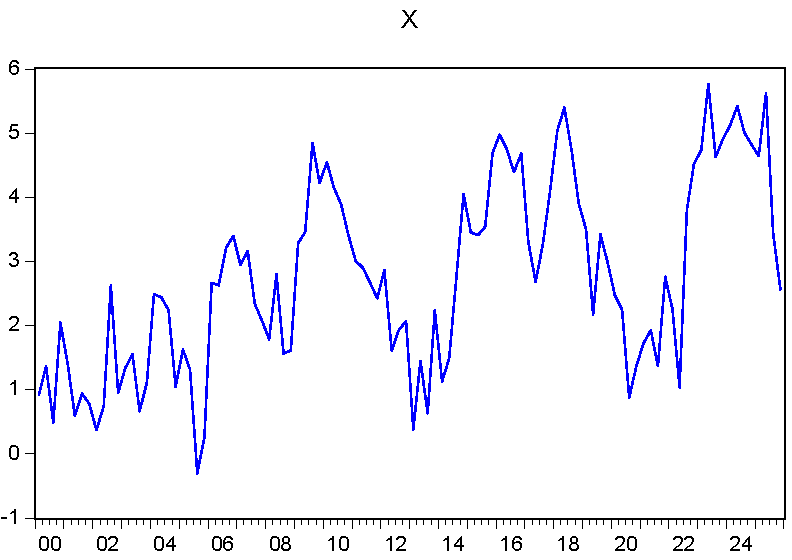
\includegraphics[width=0.25\textwidth]{test_engEviews_files/figure-latex//mychunk-grap} 

}

\caption{somefigure}\label{fig:mychunk}
\end{figure}

\begin{Shaded}
\begin{Highlighting}[]
\NormalTok{EViews}\SpecialCharTok{\textgreater{}} \FunctionTok{library}\NormalTok{(magrittr)}
\NormalTok{EViews}\SpecialCharTok{\textgreater{}} 
\NormalTok{EViews}\SpecialCharTok{\textgreater{}}\NormalTok{ mychunk}\SpecialCharTok{$}\NormalTok{page3 }\SpecialCharTok{\%\textgreater{}\%}\NormalTok{ head}
\end{Highlighting}
\end{Shaded}

\begin{verbatim}
##         date         x        y          z
## 1 2020-01-01 -1.129815 1.490471 -0.5534944
## 2 2021-01-01 -2.337099 2.742103 -1.0478218
## 3 2022-01-01 -2.907247 3.316451  0.3308785
## 4 2023-01-01 -1.464758 4.763057  1.2231814
## 5 2024-01-01 -3.776139 4.218609  0.7396137
## 6 2025-01-01 -2.974502 4.325482  0.2858918
\end{verbatim}

\begin{Shaded}
\begin{Highlighting}[]
\NormalTok{EViews}\SpecialCharTok{\textgreater{}}\NormalTok{ mychunk}\SpecialCharTok{$}\NormalTok{ols }
\end{Highlighting}
\end{Shaded}

\begin{verbatim}
##       aic df     coefs       dw        f    fprob       hq      logl  meandep
## 1 3.48178  4  2.108521 1.569123 1.071463 0.359089 3.203913 -8.445341 3.476029
## 2      NA NA -0.562391       NA       NA       NA       NA        NA       NA
##   ncoef     pval       r2    rbar2 regobs  schwarz    sddep       se      ssr
## 1     2 0.209283 0.211273 0.014091      6 3.412367 1.219507 1.210884 5.864963
## 2    NA 0.359089       NA       NA     NA       NA       NA       NA       NA
##    stderrs    tstats
## 1 1.410575  1.494796
## 2 0.543313 -1.035115
\end{verbatim}

\begin{Shaded}
\begin{Highlighting}[]
\NormalTok{EViews}\SpecialCharTok{\textgreater{}}\NormalTok{ mychunk}\SpecialCharTok{$}\NormalTok{tab}
\end{Highlighting}
\end{Shaded}

\begin{verbatim}
##           Dependent.Variable..Y           X                       X.1
## 1         Method: Least Squares                                      
## 2  Date: 06/24/22   Time: 11:38                                      
## 3             Sample: 2020 2025                                      
## 4      Included observations: 6                                      
## 5                                                                    
## 6                      Variable Coefficient                Std. Error
## 7                                                                    
## 8                             C    2.108521                  1.410575
## 9                             X   -0.562391                  0.543313
## 10                                                                   
## 11                    R-squared    0.211273        Mean dependent var
## 12           Adjusted R-squared    0.014091        S.D. dependent var
## 13           S.E. of regression    1.210884     Akaike info criterion
## 14            Sum squared resid    5.864963         Schwarz criterion
## 15               Log likelihood   -8.445341      Hannan-Quinn criter.
## 16                  F-statistic    1.071463        Durbin-Watson stat
## 17            Prob(F-statistic)    0.359089                          
## 18                                                                   
##            X.2      X.3
## 1                      
## 2                      
## 3                      
## 4                      
## 5                      
## 6  t-Statistic  Prob.  
## 7                      
## 8     1.494796   0.2093
## 9    -1.035115   0.3591
## 10                     
## 11             3.476029
## 12             1.219507
## 13             3.481780
## 14             3.412367
## 15             3.203913
## 16             1.569123
## 17                     
## 18
\end{verbatim}

\begin{Shaded}
\begin{Highlighting}[]
\NormalTok{EViews}\SpecialCharTok{\textgreater{}}\NormalTok{ mychunk}\SpecialCharTok{$}\NormalTok{mati }\SpecialCharTok{\%\textgreater{}\%}\NormalTok{ head }
\end{Highlighting}
\end{Shaded}

\begin{verbatim}
## NULL
\end{verbatim}

\hypertarget{r-plots}{%
\section{R plots}\label{r-plots}}

\begin{Shaded}
\begin{Highlighting}[]
\NormalTok{EViews}\SpecialCharTok{\textgreater{}} \FunctionTok{print}\NormalTok{(knitr}\SpecialCharTok{::}\NormalTok{opts\_current}\SpecialCharTok{$}\FunctionTok{get}\NormalTok{(}\StringTok{"sagir"}\NormalTok{))}
\NormalTok{EViews}\SpecialCharTok{\textgreater{}} \FunctionTok{print}\NormalTok{(knitr}\SpecialCharTok{::}\NormalTok{opts\_current}\SpecialCharTok{$}\FunctionTok{get}\NormalTok{(}\StringTok{"fig.show"}\NormalTok{))}
\NormalTok{EViews}\SpecialCharTok{\textgreater{}}\NormalTok{ y}\OtherTok{=}\FunctionTok{cumsum}\NormalTok{(}\FunctionTok{rnorm}\NormalTok{(}\DecValTok{100}\NormalTok{))}
\NormalTok{EViews}\SpecialCharTok{\textgreater{}}\NormalTok{ x}\OtherTok{=}\FunctionTok{cumsum}\NormalTok{(}\FunctionTok{rnorm}\NormalTok{(}\DecValTok{100}\NormalTok{))}
\NormalTok{EViews}\SpecialCharTok{\textgreater{}} 
\NormalTok{EViews}\SpecialCharTok{\textgreater{}} \FunctionTok{plot}\NormalTok{(x,y)}
\end{Highlighting}
\end{Shaded}

\begin{Shaded}
\begin{Highlighting}[]
\NormalTok{EViews}\SpecialCharTok{\textgreater{}}\NormalTok{ data}\OtherTok{=}\FunctionTok{data.frame}\NormalTok{(}\AttributeTok{y=}\FunctionTok{runif}\NormalTok{(}\DecValTok{100}\NormalTok{),}\AttributeTok{x=}\FunctionTok{runif}\NormalTok{(}\DecValTok{100}\NormalTok{))}
\NormalTok{EViews}\SpecialCharTok{\textgreater{}} \FunctionTok{eviews\_graph}\NormalTok{(data,}\AttributeTok{save\_path =} \StringTok{""}\NormalTok{,}\AttributeTok{frequency =} \StringTok{"m"}\NormalTok{,}\AttributeTok{start\_date =} \DecValTok{1990}\NormalTok{,}\AttributeTok{group =}\NormalTok{ F,}\AttributeTok{options =} \StringTok{"m"}\NormalTok{,}\AttributeTok{graph\_procs =} \StringTok{"template eviews5"}\NormalTok{)}
\end{Highlighting}
\end{Shaded}

\begin{Shaded}
\begin{Highlighting}[]
\NormalTok{EViews}\SpecialCharTok{\textgreater{}} \FunctionTok{rwalk}\NormalTok{(}\StringTok{"x y z"}\NormalTok{,}\AttributeTok{num\_observations =} \DecValTok{100}\NormalTok{,}\AttributeTok{frequency =} \StringTok{"7"}\NormalTok{,}\AttributeTok{start\_date =} \StringTok{"1"}\NormalTok{)}
\NormalTok{EViews}\SpecialCharTok{\textgreater{}} 
\NormalTok{EViews}\SpecialCharTok{\textgreater{}}\NormalTok{ eviews}\SpecialCharTok{$}\NormalTok{xyz }\SpecialCharTok{\%\textgreater{}\%}\NormalTok{ head}
\NormalTok{EViews}\SpecialCharTok{\textgreater{}} 
\NormalTok{EViews}\SpecialCharTok{\textgreater{}} \FunctionTok{eviews\_graph}\NormalTok{(eviews}\SpecialCharTok{$}\NormalTok{xyz,}\AttributeTok{group =}\NormalTok{ T,}\AttributeTok{graph\_procs =} \StringTok{"template midnight"}\NormalTok{,}\AttributeTok{graph\_command =} \StringTok{"line"}\NormalTok{)}
\end{Highlighting}
\end{Shaded}


\end{document}
